\documentclass[twocolumn]{article}
\usepackage[utf8]{inputenc}
\usepackage[margin=1in]{geometry}  % 调整页面边距
\usepackage{titling}               % 控制标题位置
\usepackage{booktabs}              % 表格宏包
\usepackage{amssymb}
\usepackage{ctex}                  % 中文支持包
\usepackage{authblk}			   % 多作者
\usepackage{graphicx}
\usepackage{ragged2e}           % 摘要两端对齐
% \usepackage{tabularx}			% 表格宽度
% \usepackage{xeCJK}
\setlength{\droptitle}{-3.0cm}     % 将标题上移3.0厘米

\title{v31 Medical Image Synthesis from CT to PET using Convolutional Neural Network}
\author[1] {Xiaoyu Deng}
\author[1,2] {Kouki Nagamune}
\author[1] {Hiroki Takada}
% \author[1] {Teacher Author}
% \author[1,3]{Third Author}
\affil[1]{University of Fukui, 3-9-1 Bunkyo, Fukui, 910-0019, Japan}
\affil[2]{University of Hyogo, 2167 Shosha, Himeji, Hyogo, 670-2280, Japan}
% \affil[3]{Research Institute, Company Z}
\date{ }

\begin{document}

\twocolumn[
	\maketitle

	\begin{center}
		\begin{abstract}
			\begin{justify}
				U-Net, a deep learning architecture, has gained widespread application in medical image processing due to its exceptional performance and efficient structural design. This architecture enhances traditional convolutional neural networks with its symmetric "U" shape, making it extensively utilized for applications such as image denoising, medical image registration, attenuation correction, lesion segmentation, and facial image restoration. This study leverages the U-Net architecture for cross-modality conversion from computed tomography to positron emission tomography images.
				Preliminary results demonstrate rapid performance improvements within the initial training epochs, achieving stability and high-quality reconstruction as training progresses. Despite observable fluctuations in performance metrics, which highlight the model's challenges in generalizing across the inherent variability of medical imaging datasets, the U-Net model exhibits robustness in image reconstruction. With further adjustments and optimizations, there is potential for enhanced performance in future applications, promising advances in the practical application of deep learning techniques in medical imaging.
			\end{justify}
		\end{abstract}
	\end{center}
	\vspace{0.5cm}  % 调整摘要与正文之间的间距
]

\section{Introduce}
% U-Net is a deep learning architecture initially designed for medical image segmentation tasks and has become widely popular in the field of medical image processing due to its outstanding performance and efficient structure. The architecture of U-Net improves upon the conventional convolutional neural network (CNN) by featuring a symmetric "U" shape, including a contracting path (encoder) and an expanding path (decoder). A key characteristic of U-Net is the use of skip connections, which connect feature maps from the contracting path to corresponding layers in the expanding path. This design enables the network to utilize more precise spatial information during the upsampling process, which is crucial for enhancing the accuracy of segmentation boundaries, particularly when precise delineation of structures in medical images is essential.

% Common strategies for increasing the scale of the U-Net model include deepening the network, expanding the number of feature map channels, refining the skip connection structure, and incorporating attention modules such as Transformer-based architectures. While these improvements can enhance model performance, they also increase model complexity and computational requirements, often encountering performance bottlenecks. In this study, we employ multiple simple encoder-decoder structures to construct a generative network and evaluate the performance of multi-stage models in medical image generation tasks.
% U-Net is a deep learning architecture initially designed for medical image segmentation tasks and has become widely popular in the field of medical image processing due to its outstanding performance and efficient structure. The architecture of U-Net is an improvement over the typical convolutional neural network (CNN), featuring a symmetric "U" shape that includes a contracting path (encoder) and an expanding (decoder) path. A key feature of U-Net is its use of skip connections, which connect feature maps from the contracting path to corresponding layers in the expanding path. Such a design allows the network to utilize more precise spatial information during the upsampling process, which is crucial for enhancing the accuracy of segmentation boundaries, especially where the delineation of structures in medical images is critically important.
U-Net 是一种最初为医学图像分割任务设计的深度学习架构,由于其出色的性能和高效的结构,在医学图像处理领域已变得非常流行。U-Net 的架构是对典型卷积神经网络(CNN)的改进,其特点是呈对称的“U”形,包括一个收缩路径(编码器)和一个扩张路径(解码器)。U-Net 的一个关键特征是它使用了跳跃连接,将来自收缩路径的特征图连接到扩张路径中的相应层。这种设计使得网络能够在上采样过程中利用更精确的空间信息,这对于提高分割边界的准确性至关重要,尤其是在医学图像中结构描绘至关重要的地方。
增加UNet模型规模的方式有增加网络深度,增加特征图通道数,改进跳跃连接结构,融入Transformer等注意力模块等。这些改进可以提高模型的性能,但也会增加模型的复杂度和计算量且往往存在性能瓶颈,本研究使用多个简单的编解码器结构构建生成网络,验证多阶模型在医学图像生成任务中的性能。
本文的主要贡献在于使用多阶级联扩展框架,使用简单编解码器模型构建多个多阶级联模型进行CT到PET图像的转换任务,通过实验验证该扩展框架对于精度提升的有效性,并展示在每个阶段的模型中,U-Net模型在医学图像生成任务中的性能表现,以及在训练和测试过程中的多项指标变化情况。我们将对比不同阶段数的U-Net模型在CT到PET图像转换任务中的性能表现,在医学图像生成中的应用潜力。具体如下:
1.本文提出一种多阶级联扩展框架,在不改变单阶编解码器模型的情况下,使用多个简单的编解码器模型构建多个多阶级联模型进行肺部CT到PET图像的转换任务。
2.在基于公开数据上构建PETCT成对图像数据集上通过实验验证该扩展框架对于精度提升的有效性,并展示在每个阶段的模型中,U-Net模型在医学图像生成任务中的性能表现,以及在训练和测试过程中的多项指标变化情况。
3.我们将多个级联扩展模型转换后的图像与真实图像的视觉对比,探索级联扩展对生成图像的视觉质量的影响。

\section{Related Works}

% Since Olaf and colleagues \cite{navab_u-net_2015} introduced U-Net, it has become widely used due to its structural advantages and excellent performance in applications such as image denoising, medical image registration, and attenuation correction. U-Net has also been applied to various other image segmentation tasks, including lesion segmentation and facial image restoration.

% Armanious et al. \cite{armanious_medgan_2020} proposed an end-to-end medical image-to-image translation framework using GAN, demonstrating its effectiveness in tasks like PET-CT translation, MR motion artifact correction, and PET image denoising.

% Singh et al. \cite{singh_automated_2023} presented an automated medical image registration method based on U-Net, using GAN to generate pseudo-CT images from non-attenuation corrected PET images, improving the efficiency and accuracy of coronary angiography registration.

% Liu et al. \cite{liu_deep_2018} developed a method for generating pseudo-CT images used for attenuation correction from single non-attenuation corrected 18F-FDG PET images.

% Du et al. \cite{du_medical_2020} reviewed six U-Net-based methods applied in medical image segmentation, including segmentation tasks for pulmonary nodules, the heart, and the brain.

% Zeng et al. \cite{zeng_swin-casunet_2022} demonstrated good performance using a two-stage cascaded U-Net in facial image restoration tasks, suggesting that multi-stage cascaded U-Nets hold potential advantages in image generation tasks.

% Singh and Liu et al. applied U-Net architectures by fine-tuning modules for medical image registration and attenuation correction, achieving promising results in specialized domains.

% While Armanious and Zeng et al. employed cascaded U-Net structures, they did not explore the performance of multi-stage cascaded U-Nets in medical image generation tasks.

% This research utilizes a multi-stage cascaded U-Net model for CT-to-PET image translation and evaluates model performance based on the following metrics.

\begin{figure*}[t!]
	\centering
	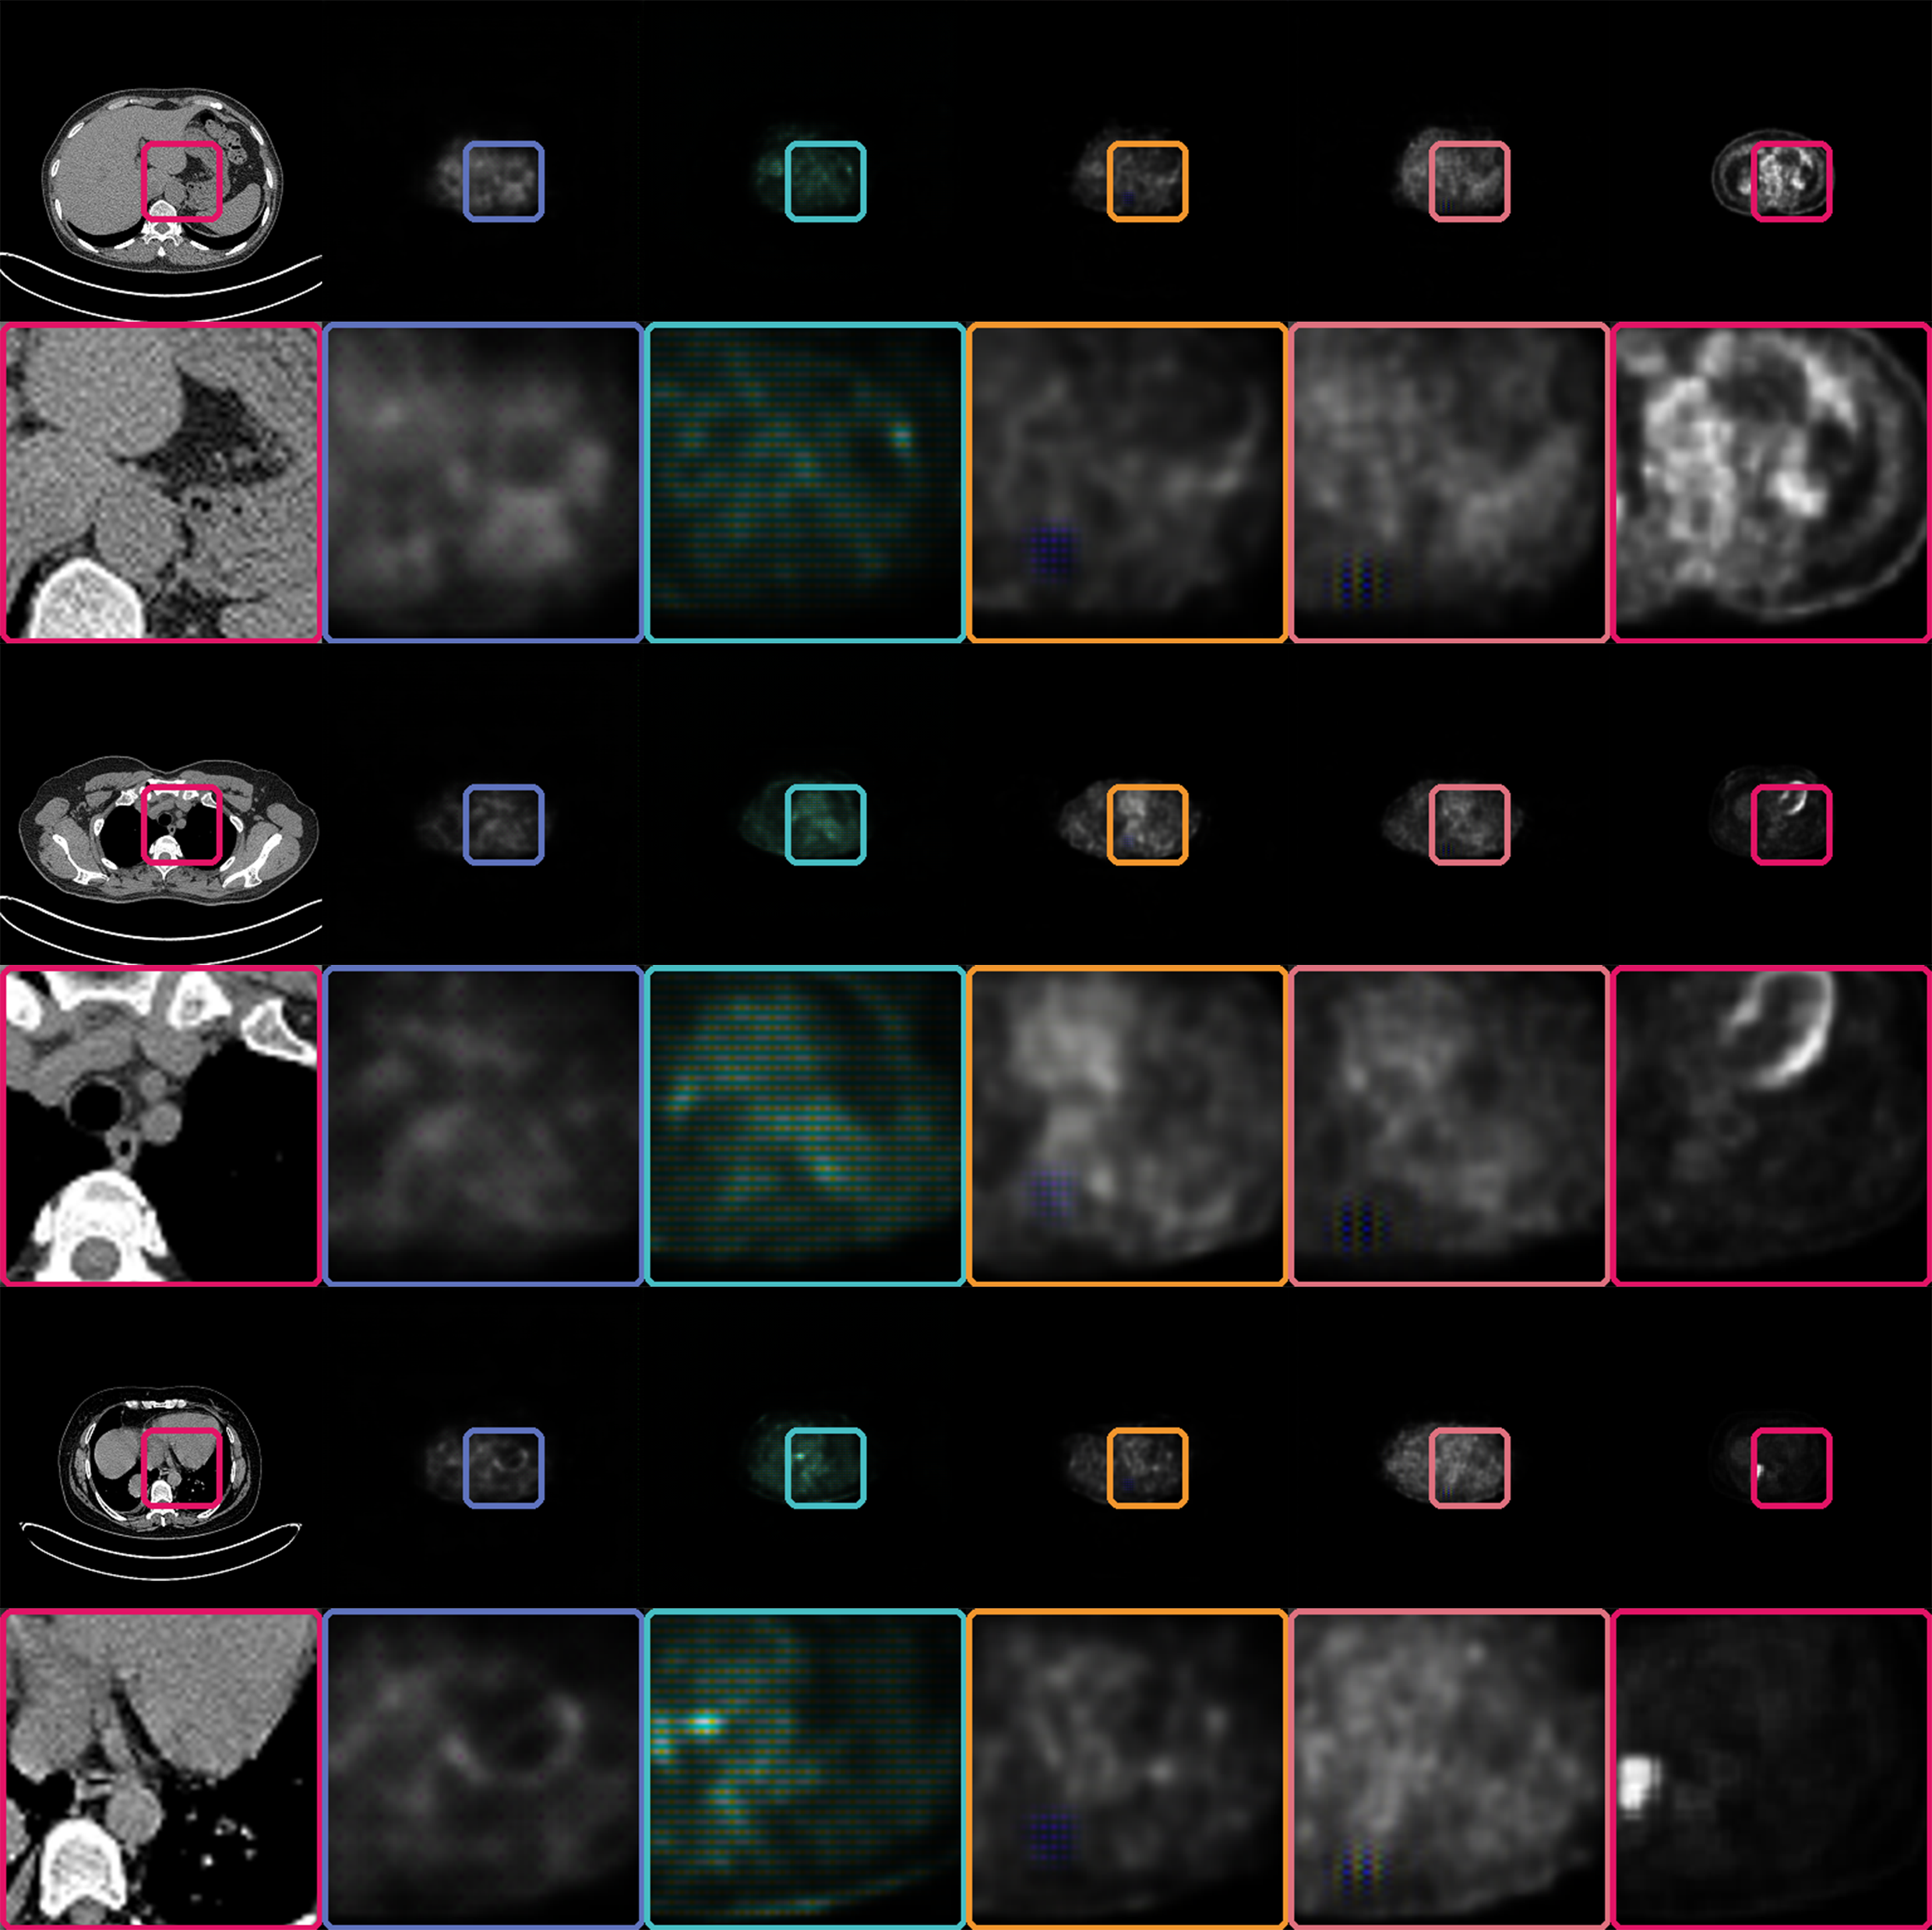
\includegraphics[width=1.0\linewidth]{u-net/lung/lung_compare.png}
	\caption[lung_compare]{Gennerated PET Image and Real CT PET Image}
	\label{fig:lung_compare}
\end{figure*}

自 Olaf 及其同事 \cite{navab_u-net_2015} 引入 U-Net 以来,由于其结构优势和在图像去噪、医学图像配准和衰减校正等应用中的出色性能,U-Net 已被广泛使用。它还应用于各种其他图像分割任务,包括病变分割,面部图像修复。
Armanious等人\cite{armanious_medgan_2020}提出了一种用于医学图像到图像的端到端框架,构建的GAN在PET-CT翻译,MR运动伪影校正和PET图像去噪等任务中验证了其性能。
Singh等人\cite{singh_automated_2023}提出了一种基于U-Net的自动化医学图像配准方法,通过GAN从未进行衰减矫正的PET图像生成伪CT图像,提高冠状动脉血管造影的配准效率和准确性。
Liu等人\cite{liu_deep_2018}开发了一种可从单个未经衰减校正的18F-FDG PET图像生成用于衰减校正的伪CT图像。
Du等人\cite{du_medical_2020}综述了六种基于U-Net结构的方法在医学图像分割中的应用,包括肺部结节分割、心脏分割、脑部分割等。
Zeng等人\cite{zeng_swin-casunet_2022}在面部图像修复任务中使用2阶级联的U-Net,展示了良好的性能,这表明多阶级联的U-Net在图像生成任务中具有潜在的优势。
Singh和Liu等人将通过微调模块的方式将模型应用在医学图像配准和衰减校正任务中,在专项领域内取得不错的效果。
Armanious和Zeng等人的工作使用了级联U-Net结构,但是并未探索多阶级联U-Net在医学图像生成任务中的性能。
本研究将使用多阶级联U-Net模型进行CT到PET图像的转换任务,并通过以下指标评估模型的性能。

结构相似性指数(SSIM)是一种复杂的指标,用于测量两幅图像之间的结构相似性。它考虑了图像的亮度、对比度和结构信息等因素。SSIM 值范围从 -1 到 1,其中 1 表示完全相似。该指标在医学图像分割中特别有用,因为它详细反映了图像的视觉和结构质量。

多尺度结构相似性指数(MS-SSIM)是 SSIM 的扩展,它跨多个尺度评估图像相似性,从而更全面地评估图像质量。这在处理分辨率差异很大的医学图像时特别有用。

峰值信噪比(PSNR)是另一种广泛用于测量图像重建质量的指标。它用于图像和视频压缩以及其他形式的信号处理等领域,通过比较原始图像和处理后图像之间的相似性来评估图像重建或压缩的质量。

平均绝对误差(MAE)是评估图像重建质量最常用的指标之一。它计算的是重建图像与原始图像之间像素强度差异的绝对值的平均值。MAE 值越低,图像重建中的误差越小,质量越高。与均方误差(MSE)相比,MAE 对异常值不敏感。在医学图像处理中,MAE 可以用于评估医学图像重建和分割算法的性能。在pytorch框架下,像素会被缩放到0到1之间,因此与MSE相比,MSE的值会更小,在一定程度上影响了轻视了像素误差的影响。因此本文选择MAE作为评估指标之一。


% Since its introduction by Olaf and colleagues \cite{navab_u-net_2015}, U-Net has been widely used due to its structural advantages and excellent performance in applications such as image denoising \cite{armanious_medgan_2020}, medical image registration \cite{singh_automated_2023}, and attenuation correction \cite{liu_deep_2018}. It is also applied to various other image segmentation tasks including lesion segmentation \cite{du_medical_2020} and face image restoration \cite{zeng_swin-casunet_2022}.

% In experiments using U-Net or other image segmentation and reconstruction models, it is crucial to evaluate the accuracy, reliability, and effectiveness of the model's performance. Various quantitative metrics commonly used in U-Net related experiments help researchers and developers understand the model's performance in specific tasks.

% The Structural Similarity Index Measure (SSIM) is a complex metric used to measure the structural similarity between two images. It considers aspects such as luminance, contrast, and structural information of the images. The SSIM value ranges from -1 to 1, where 1 indicates perfect similarity. This metric is particularly useful in medical image segmentation as it provides a detailed reflection of the visual and structural quality of the images.

% The Multi-Scale Structural Similarity Index Measure (MS-SSIM) is an extension of SSIM that evaluates image similarity across multiple scales, offering a more comprehensive assessment of image quality. This is especially useful when dealing with medical images that vary significantly in resolution.


% Peak Signal-to-Noise Ratio (PSNR) is another widely used metric to measure the quality of image reconstruction. It is employed in fields like image and video compression and other forms of signal processing to assess the quality of an image reconstruction or compression by comparing the similarity between the original and processed images.

% Mean Squared Error (MSE) is one of the most commonly used metrics to evaluate the quality of an image reconstruction. It calculates the average of the squares of the pixel intensity differences between the reconstructed image and the original image. The lower the MSE value, the smaller the error in image reconstruction and the higher the quality.

% This study will utilize the standard U-Net model to perform cross-modality conversion tasks from CT to PET images and demonstrate the model's performance using the above metrics.

\section{Method}
Encoder-decoder architecture is designed symmetrically, with a contracting path to capture context and a symmetric expanding path that enables precise localization. This study aims to construct a standard U-Net, a convolutional neural network, to develop a cross-modality medical image converter from CT to PET images. The model will be optimized using a specific loss function suitable for this type of image conversion task.
本文级联扩展框架使用网络主要包括编码器块,解码器块,以及一个可视化块。编码器块用于提取输入图像的特征,解码器块用于将特征图转换为输出图像。可视化块用于将输出图像转换为可视化格式。单个编解码器的结构如图\ref{fig:Encoder_Decoder_Pair}所示。

% % TODO: \usepackage{graphicx} required
\begin{figure*}[t!]
	\centering
	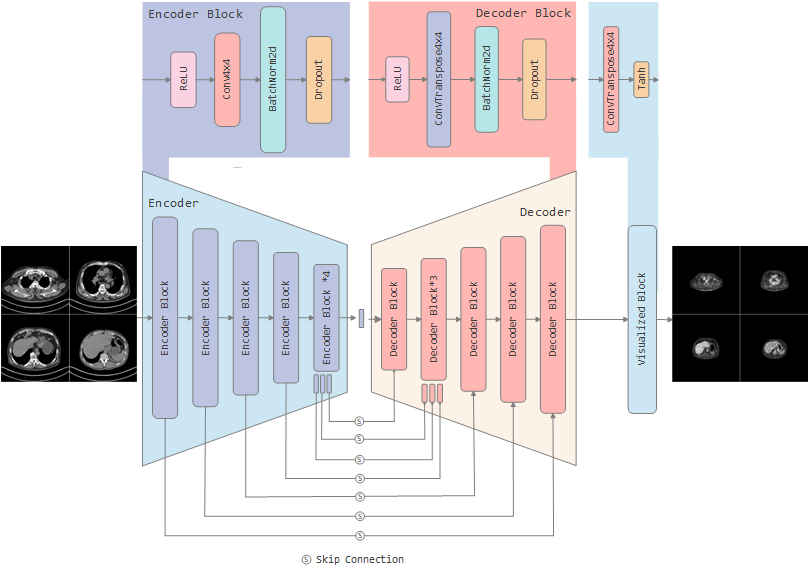
\includegraphics[width=1.0\linewidth]{u-net/lung/Encoder-Decoder-5layer-250406}
	\caption[architecture]{Schematic Diagram of Data Flow Within the Model. The PET image is shown on the left, and the CT image on the right. The blue modules correspond to the encoder architecture, while the orange modules represent the decoder architecture. The upper portion of the figure illustrates the fundamental structures of the encoder blocks, decoder blocks, and visualization blocks. The connections in the lower portion indicate the skip connections.}
	\label{fig:Encoder_Decoder_Pair}
\end{figure*}

\textbf{Encoder Block} The encoder follows the typical architecture of a convolutional network. It consists of repeated application of two $3\times3$ convolutions, each followed by a rectified linear unit (ReLU) and a $2\times2$ max pooling operation with stride 2 for downsampling. At each downsampling step, the number of feature channels is doubled. The convolution operation in U-Net can be described by the following equation:
\[
	I' = \sum_{i,j} (I * K)(i,j) + b
\]
where \(I\) represents the input image, \(K\) is the convolution kernel, \(b\) is the bias, and \(I'\) is the output feature map.


% Max pooling in the encoder is used to reduce the spatial dimensions of the input feature maps:
% \[
% 	P(x,y) = \max(I(x + i, y + j))
% \]
% where \(P(x,y)\) is the pooled output, and \(I(x + i, y + j)\) represents the input in the neighborhood around location \((x, y)\).

\textbf{Decoder Block} The decoder includes a series of upsampling and convolution operations. Each step in the expanding path includes an upsampling of the feature map followed by a $2\times2$ convolution that halves the number of feature channels, a concatenation with the correspondingly cropped feature map from the contracting path, and two $3\times3$ convolutions, each followed by a ReLU. Up sampling in the expanding path uses transposed convolutions to increase the size of the feature map:
\[
	U = K^T * I
\]
where \(K^T\) is the transposed convolution kernel and \(U\) is the upsampled output.

\textbf{Visual Block} The visual block is 一个变形的解码器块,主要用于将输出图像转换为可视化格式。它的结构与解码器块类似,但没有跳跃连接,并且使用的非线性函数不同。它的作用是将解码器块的输出转换为最终的可视化图像。

\begin{table}[h]
	% \centering
	\caption{Encoder-decoder Setting Table}
	\label{tab:encoder_setting}
	\begin{tabular}{ccccc}
		\hline
		Block Name   & input & output & trans & dropout \\
		\hline
		Encoder 1    & 3     & 64     & -     & -       \\
		Encoder 2    & 64    & 128    & -     & -       \\
		Encoder 3    & 128   & 512    & -     & -       \\
		Encoder 4    & 256   & 512    & -     & -       \\
		Encoder 5    & 512   & 512    & -     & -       \\
		Encoder 6    & 512   & 512    & -     & -       \\
		Encoder 7    & 512   & 512    & -     & -       \\
		Encoder 8    & 512   & 512    & -     & -       \\
		Decoder 1    & 512   & 1024   & 512   & 0.5     \\
		Decoder 2    & 1024  & 1024   & 512   & 0.5     \\
		Decoder 3    & 1024  & 1024   & 512   & 0.5     \\
		Decoder 4    & 1024  & 1024   & 512   & -       \\
		Decoder 5    & 1024  & 512    & 256   & -       \\
		Decoder 6    & 512   & 256    & 128   & -       \\
		Decoder 7    & 256   & 128    & 64    & -       \\
		Visual Block & 128   & 3      & -     & -       \\
		\hline
	\end{tabular}
\end{table}

\subsection{级联扩展框架}
本文中的级联扩展框架使用前文的编解码器作为基本单元,将多个编解码器级联在一起,形成一个多阶级联的网络结构。每个编解码器的输出都作为下一个编解码器的输入,从而实现了多阶级联的效果。该框架的设计旨在通过级联多个编解码器来提高模型的性能和准确性。将前一个编解码器的输出作为下一个编解码器的输入,可以使模型在每个阶段都能够学习到更丰富的特征信息,从而提高最终生成图像的质量。这里可以使用不同阶段的输出计算损失函数从而分段优化模型,这里本文不作深入考虑。本文构建了10个不同的级联编解码器模型,以及引入了1个包含密集连接和分段优化的模型,称为DualSGAN。该模型的结构与前面的级联扩展框架类似,但在每个阶段的输出上都引入了密集连接和分段优化。通过这种方式,DualSGAN能够更好地捕捉不同阶段的特征信息,从而提高模型的性能和准确性。表\ref{tab:model_parameters}展示了不同模型的参数数量.

\begin{table}[h]
	\centering
	\caption{Parameters of Neural Networks.}
	\label{tab:model_parameters}
	\begin{tabular}{ccccc}
		\hline
		Architectures & Parameters \\
		\hline
		Stage01       & 54.41      \\
		Stage02       & 108.82     \\
		DualSG      & 92.54      \\
		Stage03       & 163.24     \\
		Stage04       & 217.66     \\
		Stage05       & 272.07     \\
		Stage06       & 326.49     \\
		Stage07       & 380.90     \\
		Stage08       & 435.31     \\
		Stage09       & 489.73     \\
		Stage10       & 544.155    \\
		\hline
		\multicolumn{2}{p{201pt}}{The table depicts the Parameters of different generators. The quantity of parameters is expressed in millions.}
	\end{tabular}
\end{table}


\section{Experiments}
This study employs the encoder-decoer architecture for cross-modality medical image conversion tasks, specifically to construct a U-Net that inputs a CT image and converts it into a corresponding PET image. In this research, the lung PET or CT scan data were powered by the National Cancer Institute Cancer Imaging Program (CIP) \cite{li_large-scale_2020}.  The dataset encompasses 251,135 lung scan images from 355 subjects, primarily collected between 2009 and 2011, including each subject's gender, age, weight, smoking history, and cancer diagnosis classification. All scan data in the dataset are stored in DICOM format. This study processed these 251,135 scan data using the MicroDicom software on a Windows operating system. The subjects in the dataset are labeled according to the type of cancer: Type A for adenocarcinoma, Type B for small cell carcinoma, Type E for large cell carcinoma, and Type G for squamous cell carcinoma. Not all subjects' data include both PET and CT scans. Therefore, this study selected only the scan data of 38 subjects diagnosed with small cell carcinoma (Type B), which include PET scans, various CT scans, and fusion-enhanced scan images. 具体的提取方法来自我们另外一份尚未发布的研究内容。 我们最终取得了464对PET/CT图像数据,包含928张图像。In this study, 我们将这些图像数据分为训练集和测试集,训练集包含800张图像,测试集包含128张图像。The specific division of the dataset is shown in the following table\ref{tab:dataset_partition_1}.

% 插入三线表
\begin{table}[h]
	\centering
	\caption{Dataset Partition of Experiment}
	\label{tab:dataset_partition_1}
	\begin{tabular}{cccc}
		\toprule
		Params count     & Test & Train & Total \\
		\midrule
		Lung PET/CT Pair & 64   & 400   & 464   \\
		Total Images     & 128  & 800   & 928   \\
		\bottomrule
	\end{tabular}
\end{table}

In this experiment, the standard encoder-decoder model is employed to synthesize positron emission tomography images from computed tomography images as inputs. 我们使用常见的MSE和对抗损失来优化我们的生成对抗网络。 The model optimizer used is the Adam optimizer, with a learning rate (lr) set at 0.001. This relatively low learning rate assists the model in steadily approaching the global optimum during the training process. The best experimental results are shown in Table \ref{tab:exps_result}. 

\begin{table}[h]
	\centering
	\caption{Max SSIM,PSNR,MAE Results of Experiment}
	\label{tab:exps_result}
	\begin{tabular}{cccc}
		\toprule
		Stage Count & SSIM            & PSNR             & MAE             \\
		\midrule
		1 Stage     & 0.9149          & 27.7411          & 0.0119          \\
		2 Stages    & 0.9182          & 27.9950          & 0.0109          \\
		3 Stages    & 0.9060          & 27.6395          & 0.0127          \\
		4 Stages    & 0.9155          & 28.1969          & 0.0112          \\
		5 Stages    & 0.9104          & 26.6691          & 0.0130          \\
		6 Stages    & 0.9167          & 27.9794          & 0.0108          \\
		7 Stages    & \textbf{0.9255} & 27.1919          & 0.0116          \\
		8 Stages    & 0.9178          & 28.5503          & 0.0107          \\
		9 Stages    & 0.9093          & 28.7770          & 0.0109          \\
		10 Stages   & 0.9245          & \textbf{28.9168} & \textbf{0.0097} \\
		DualSGAN    & 0.9122          & 28.7630          & 0.0105          \\
		\bottomrule
	\end{tabular}
\end{table}

此外,我们的实验针对每个模型记录了超过 200 个训练轮次的数据,包括结构相似性指数、峰值信噪比 (PSNR) 和均方误差 (MSE)。在每个轮次后都进行了测试,损失、训练和测试的 SSIM、PSNR 和 MAE 指标的变化如各自的图所示。该模型在训练集和测试集上都表现出了值得称赞的性能。

% \begin{table*}[h]
% 	\centering
% 	\caption{SSIM,PSNR,MAE Results of Experiment}
% 	\label{tab:exp_result}
% 	\begin{tabular}{ccccc}
% 		\toprule
% 		Stage Count & SSIM          & PSNR           & MAE           \\
% 		\midrule
% 		1 Stage     & 0.9072±0.0115 & 26.9875±0.9426 & 0.0128±0.0012 \\
% 		2 Stages    & 0.9085±0.0285 & 27.2766±1.4067 & 0.0118±0.0020 \\
% 		3 Stages    & 0.8783±0.0514 & 26.3093±1.1418 & 0.0143±0.0023 \\
% 		4 Stages    & 0.8830±0.1388 & 26.6404±1.7853 & 0.0133±0.0035 \\
% 		5 Stages    & 0.8951±0.0501 & 26.0332±0.5600 & 0.0145±0.0021 \\
% 		6 Stages    & 0.9031±0.1055 & 26.1884±2.5253 & 0.0134±0.0037 \\
% 		7 Stages    & 0.9154±0.0483 & 25.8576±1.5094 & 0.0135±0.0028 \\
% 		8 Stages    & 0.8859±0.2105 & 27.5697±2.7027 & 0.0127±0.0089 \\
% 		9 Stages    & 0.8771±0.1441 & 27.1008±3.1234 & 0.0133±0.0045 \\
% 		10 Stages   & 0.9102±0.0656 & 27.9325±1.9125 & 0.0108±0.0032 \\
% 		\bottomrule
% 	\end{tabular}
% \end{table*}




% TODO: \usepackage{graphicx} required
\begin{figure}[h]
	\centering
	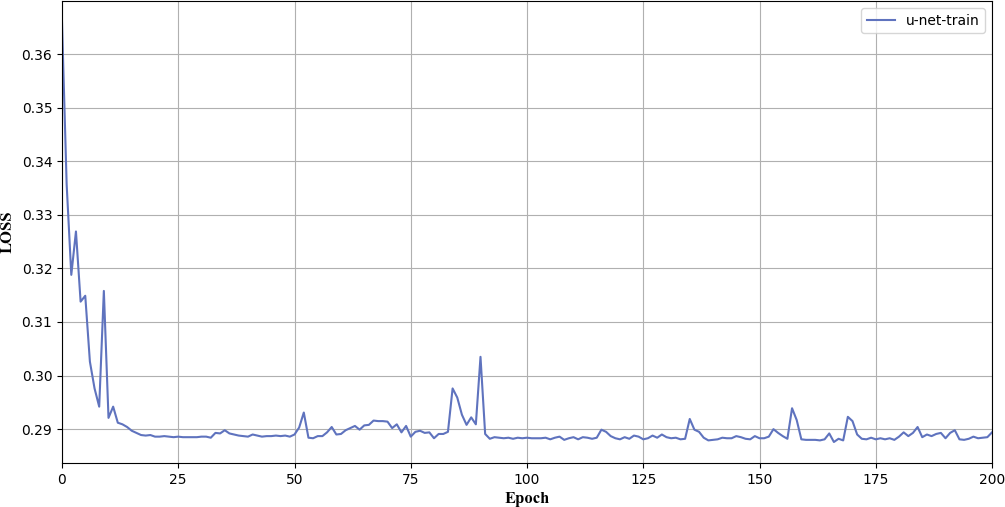
\includegraphics[width=1.0\linewidth]{u-net/LOSS}
	\caption[loss_train]{Loss Line Figure of All Epoch in Train Process}
	\label{fig:loss_train}
\end{figure}

Figure \ref{fig:loss_train} shows that during the initial few training epochs, the loss rapidly decreases from approximately 0.36 to close to 0.29. This indicates that the model quickly improved its fit to the training data, making the learning process highly effective during this stage. After the rapid decline, the loss values tend to stabilize, fluctuating around 0.29. This trend suggests that the model may have reached a stable state in its training, where further learning yields limited performance improvements. Although the loss values are relatively stable, there are still minor fluctuations at certain epochs, such as around the 50th, 100th, and 175th epochs. These fluctuations could be due to random factors in the training process, such as random selection of batch data, adjustments in the learning rate, or external disturbances. Overall, the loss values remain relatively low and stable over 200 training epochs, indicating that the model possesses a certain degree of generalization ability and has maintained good stability throughout the training process.


\begin{figure}[h]
	\centering
	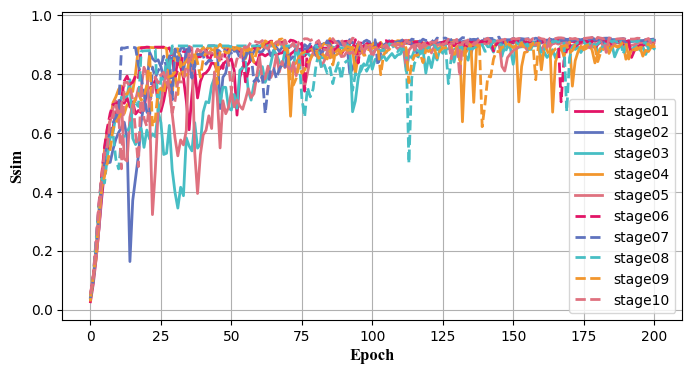
\includegraphics[width=1.0\linewidth]{u-net/lung/csv_img_in_1_img_8_4/ssim_comparison}
	\caption[ssim]{SSIM Line Figure of All Epoch in Train and Test Process}
	\label{fig:ssim}
\end{figure}

Figure \ref{fig:ssim} shows that the SSIM values rapidly increase during the initial training phase (first 25 epochs), rising from near zero to above 0.6. This indicates that the U-Net model quickly learned the mapping relationship between CT and PET images, showing significant initial learning effects. After this rapid growth, the SSIM values on both the training and testing sets tend to stabilize, mainly fluctuating around 0.7. This demonstrates that the model maintained high image reconstruction quality during the continued training process. Throughout the training period, the SSIM values on the training set are usually higher than those on the testing set, which might be a sign of slight overfitting, suggesting that the model may be overly optimized for the training data and slightly less generalized for unseen test data.


\begin{figure}[h]
	\centering
	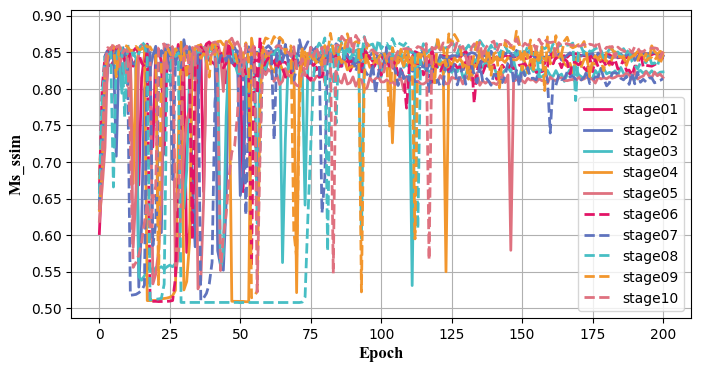
\includegraphics[width=1.0\linewidth]{u-net/lung/csv_img_in_1_img_8_4/ms_ssim_comparison}
	\caption[msssim]{MS-SSIM Line Figure of All Epoch in Train and Test Process}
	\label{fig:msssim}
\end{figure}

Figure \ref{fig:msssim} illustrates that, for both the training and testing datasets, the MS-SSIM values rapidly improve within the initial few epochs. This shows that the model effectively captured the key features and structural information necessary for the conversion from CT to PET images early in the learning process. After the initial rapid improvement, the MS-SSIM values enter a phase of more stable fluctuations, as reflected in both the training and testing data. The MS-SSIM values for the training data are slightly higher than those for the testing data, a common phenomenon in machine learning models, which may indicate slight overfitting. After about 50 epochs, despite some fluctuations, the MS-SSIM values generally remain at a high level, especially above 0.7, indicating that the model has a good ability to capture the structural similarity of the images. The MS-SSIM values on the testing dataset are generally slightly lower than those on the training dataset, but the gap between them is small, indicating that the model also performs well on unseen data.

\begin{figure}[h]
	\centering
	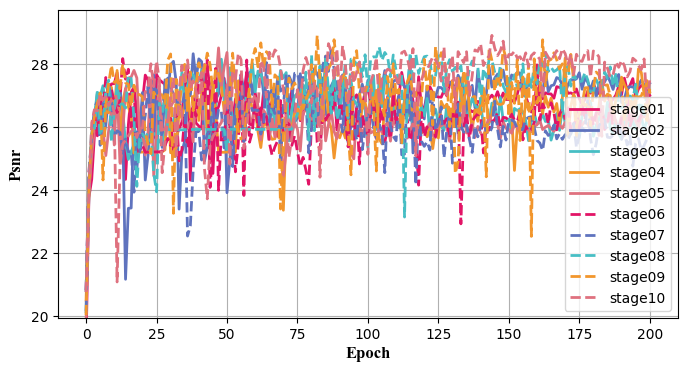
\includegraphics[width=1.0\linewidth]{u-net/lung/csv_img_in_1_img_8_4/psnr_comparison}
	\caption[psnr]{PSNR Line Figure of All Epoch in Train and Test Process}
	\label{fig:psnr}
\end{figure}

Figure \ref{fig:psnr} displays that, for both training (blue line) and testing (red line) sets, the Peak Signal-to-Noise Ratio (PSNR) values rapidly increase during the initial epochs, suggesting that the model quickly begins to effectively reconstruct PET images from CT images. The rapid improvement initially may be related to swift adjustments in the model parameters, significantly enhancing the quality of the reconstructed images. Following the initial growth, the PSNR values tend to stabilize but exhibit several significant fluctuations during both training and testing processes. These fluctuations might reflect changes in performance when the model encounters difficult samples within the data or due to optimization algorithms (such as learning rate adjustments). Despite these fluctuations, PSNR generally remains at a relatively high level, indicating that the model reconstructs PET images well and shows consistent performance throughout the training and testing periods. The PSNR curves for the training and testing sets are very close, indicating good generalization capability of the model to unseen data. Nonetheless, the testing curve occasionally dips below the training curve, which might be due to particularly challenging image samples in the test set.

\begin{figure}[h]
	\centering
	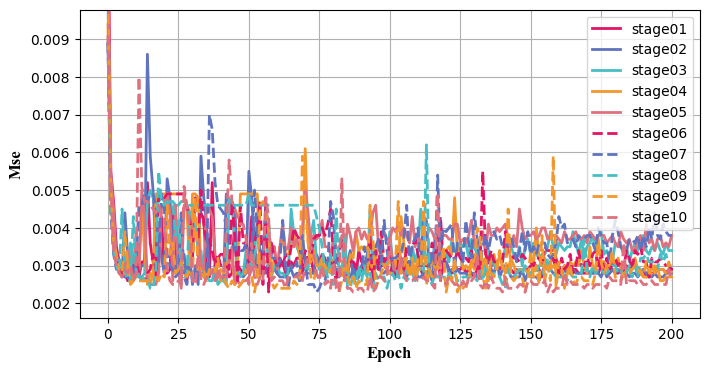
\includegraphics[width=1.0\linewidth]{u-net/lung/csv_img_in_1_img_8_4/mse_comparison}
	\caption[mse]{MSE Line Figure of All Epoch in Train and Test Process}
	\label{fig:mse}
\end{figure}

From Figure \ref{fig:mse}, it can be observed that the Mean Squared Error (MSE) for both the training and testing sets rapidly decreases from initial values of around 0.20 to below 0.05 during the initial few epochs. This indicates that the model quickly and effectively adapts to the image conversion from CT to PET, with a rapid learning rate. After the quick decline, the training and testing MSE tend to stabilize, although there are several pronounced peaks, particularly around the 125th and 175th epochs. These peaks may reflect performance fluctuations when the model processes certain specific data batches or anomalous image samples. Besides occasional peaks, MSE remains at a low level most of the time, showing relative stability of the model throughout the training and testing processes. This suggests that the model can reliably reconstruct images in most cases. The MSE curves for the training and testing sets are very close, indicating good generalization capability of the model to unseen data. This close trend also suggests that there are no significant issues with overfitting.

\begin{figure}[h]
	\centering
	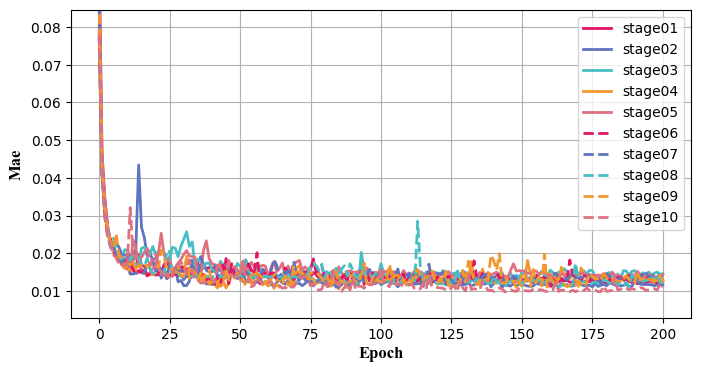
\includegraphics[width=1.0\linewidth]{u-net/lung/csv_img_in_1_img_8_4/mae_comparison}
	\caption[mae]{MAE Line Figure of All Epoch in Train and Test Process}
	\label{fig:mae}
\end{figure}


\section{Conclusion}
This research thoroughly explores the development history, technical principles, and practical applications of U-Net, and conducts an empirical study in medical image classification tasks. The experimental results demonstrate that the U-Net model shows high efficiency and stability in the task of converting CT to PET images. With further adjustments and optimizations, it is hoped that even better performance can be achieved in future applications.

\section*{Acknowledage}
We would like to express our sincere gratitude to the National Cancer Institute Cancer Imaging Program for generously making their high-quality medical imaging dataset available and authorized for use on the Internet, providing indispensable resources for the smooth conduct of this research.

\bibliographystyle{unsrt}
\bibliography{unet_ref}

\end{document}
